\chapter{Simulações}
\label{cap:III}
\section{Introdução}
 Neste capítulo mostrarei resoluções de algumas aproximações de funções e resolução de equações diferenciais utilizando métodos discutidos anteriormente. Todas as figuras obtidas aqui e implementação dos métodos foram feitas a partir da linguagem \emph{Julia}.

\section{Convergência do erro de interpolação utilizando o método espectral}
	Vamos agora ver a convergência do erro da aproximaçãode uma função de runge $\frac{1}{1+x^2},\ x\ \in [-5,5]$, para pontos \emph{equidistantes} e pontos igualmente espaçados, utilizando o polinômio de \textbf{Lagrange}.
	As aproximadas obtidas para raízes equidistantes e raízes de chebishev são:\\
\begin{figure}[!ht]
  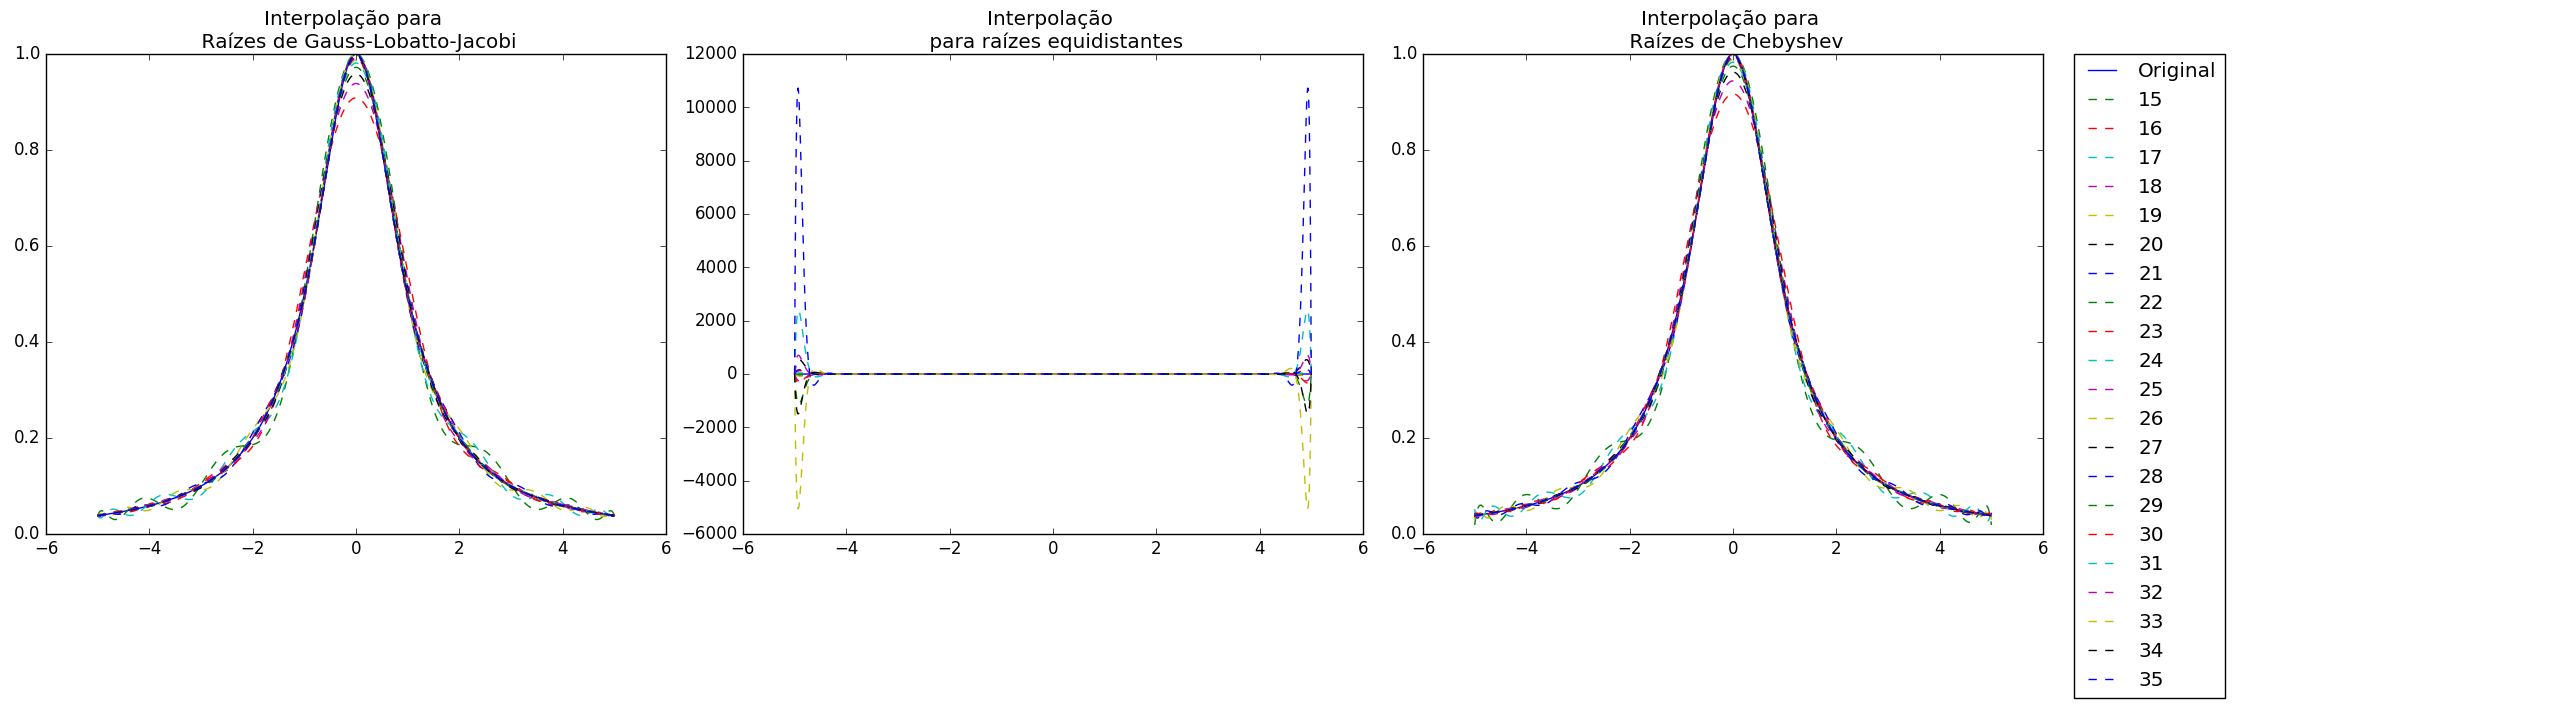
\includegraphics[width=0.8\textwidth,center]{figuras/interpolacao_todas.png}
  \caption{interpolação de polinômios de alta ordem com raízes de Gauss-Lobatto-Jacobi, igualmente espaçados, Chebyshev}
\end{figure}
Notamos novamente que para diferentes  polinômios de lagrange de alta ordem utilizando pontos igualmente espaçados, a aproximação nos pontos próximos das extremidades um erro  grande, enquanto que para pontos distribuídos usando as raízes de Chebyshev e de Gauss-Lobatto-Jacobi se comportam bem nessas regiões. Agora, iremos verificar a convergência desse erro, analizando o erro máximo para cada escolha de raízes.

\pagebreak
\begin{table}[h]
\centering
\caption{tabela de erros máximos para os diferentes tipos de raízes}
\label{my-label}
\begin{tabular}{|l|l|l|l|}
\hline
Grau & equidist & glj       & chebyshev     \\ \hline
15   & 7.19     & 4.925e-02 & 4.660e-02 \\
16   & 2.11     & 9.128e-02 & 8.309e-02 \\
17   & 14.39    & 3.480e-02 & 3.261e-02 \\
18   & 4.22     & 6.138e-02 & 5.590e-02 \\
19   & 29.19    & 2.417e-02 & 2.249e-02 \\
20   & 8.58     & 4.126e-02 & 3.758e-02 \\
\vdots   & \vdots              & \vdots    & \vdots    \\
30   & 333.94   & 5.651e-03 & 5.154e-03 \\
31   & 2384.73  & 2.229e-03 & 2.061e-03 \\
32   & 704.08   & 3.797e-03 & 3.463e-03 \\
33   & 5058.99  & 1.510e-03 & 1.402e-03 \\
34   & 1494.38  & 2.551e-03 & 2.328e-03 \\
35   & 10719.90 & 1.025e-03 & 9.488e-04 \\ \hline
\end{tabular}
\end{table}
Comparando as escolhas de raízes dos problemas conseguimos ver que a convergência do erro usando as raízes equidistantes aumenta conforme o grau do polinômio aumenta. Enquanto que para as raízes de Chebyshev e Gauss-Lobatto-Jacobi, os erros convergem algebricamente.
\begin{figure}[!ht]
  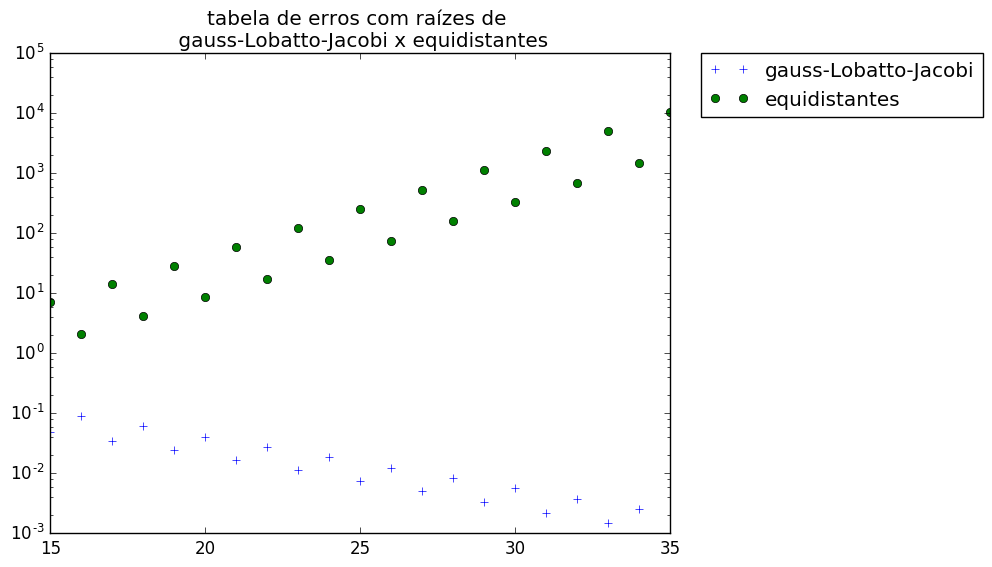
\includegraphics[width=0.5\textwidth,center]{figuras/glj_equi.png}
  \caption{comparação semilog  dos erros e graus de liberdade de raízes de glj versus equidistante }
\end{figure}
\begin{figure}[!hb]
  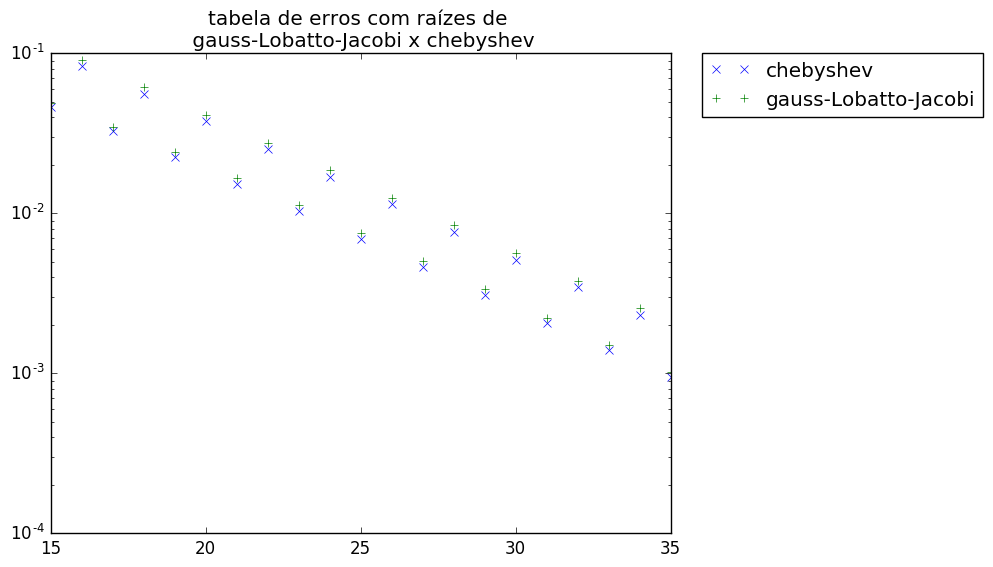
\includegraphics[width=0.5\textwidth,center]{figuras/glj_cheb.png}
  \caption{comparação semilog  dos erros e graus de liberdade de raízes de glj versus Chebyshev}
\end{figure}
\\
Notamos que embora a convergência, utilizando ambas as raízes dos polinômios, tenham o mesmo comportamento, podemos observar que como demonstrado  anteriormente a escolha do Polinômio de Chebyshev é o que melhor aproxima a função do fenômeno de Runge observando uma inclinação menor do erro.

\subsection{Convergência do erro de interpolação utilizando método H}
 Tendo aproximado a função de runge acima, utilizaremos um novo método chamado método H,método no qual subdividimos o problema em $n$ elementos de tamanho $H$. Iremos comparar o efeito desse método contra o método espectral anterior utilizando as mesmas raízes de aproximação, Gauss-Lobatto-Jacobi.

\begin{figure}[!ht]
  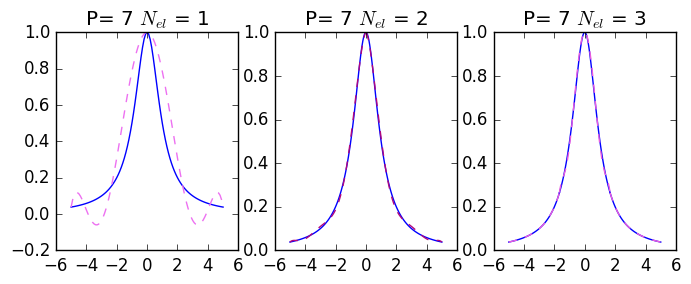
\includegraphics[width=0.8\textwidth,center]{figuras/interp_usando_FEM.png}
  \caption{gráficos das aproximações fixado o grau do polinômio em 7 e subdividimos o domínio em $N_{el}$ elementos }
\end{figure}
\begin{figure}[!hb]
  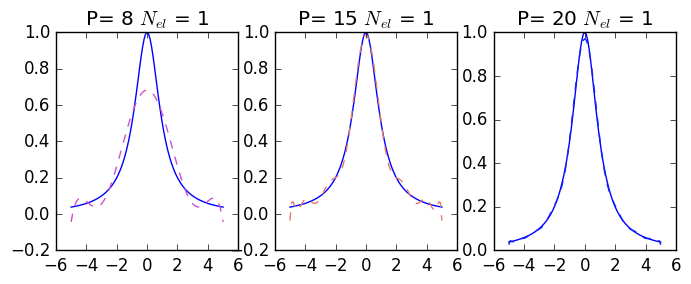
\includegraphics[width=0.8\textwidth,center]{figuras/interp_usando_FEMfixo.png}
  \caption{gráficos das aproximações fixado o número de elementos em 1 e utilizamos polinômios de grau elevado}
\end{figure}
tabela:
\begin{table}[]
\centering
\caption{Tabela de erros para a interpolação com apenas o aumento do grau de polinômio}

\label{my-label}
\begin{tabular}{|l|l|}
\hline
\multicolumn{2}{|c|}{elemento fixo} \\
\hline
erro        & Graus de liberdade   \\
6.462e-01   & 3.0                  \\
8.013e-01   & 4.0                  \\
4.385e-01   & 5.0                  \\
6.034e-01   & 6.0                  \\
2.905e-01   & 7.0                  \\
4.285e-01   & 8.0                  \\
1.884e-01   & 9.0                  \\
2.954e-01   & 10.0                 \\
1.212e-01   & 11.0                 \\
2.008e-01   & 12.0                 \\
7.699e-02   & 13.0                 \\
1.356e-01   & 14.0                 \\
4.899e-02   & 15.0                 \\
9.129e-02   & 16.0                 \\
3.477e-02   & 17.0                 \\
6.139e-02   & 18.0                 \\
2.376e-02   & 19.0                 \\
4.126e-02   & 20.0                \\
\hline
\end{tabular}
\end{table}

\begin{table}[]
\centering
\caption{Tabela de erros para a interpolação com o grau de polinômio fixo em 7 e o aumento do número de elementos}
\label{my-label}
\begin{tabular}{|l|l|l|}
\hline
\multicolumn{2}{|c|}{Polinômio Fixo} &           \\
\hline
erro         & Graus de liberdade    & $N_{el}$ \\
2.905e-01    & 7.0                 & 1         \\
1.773e-02    & 13.0                & 2         \\
2.044e-02    & 19.0                & 3         \\
2.292e-03    & 25.0                & 4         \\
2.275e-03    & 31.0                & 5        \\
\vdots       &  \vdots             & \vdots   \\
\hline
\end{tabular}
\end{table}

 Notamos nas tabelas  que para o método utilizando o grau do polinômio fixo, a convergência de seu erro é mais rápida  e seu erro já é menor para um número de elementos não muito elevado. No caso, para um número de elementos 4 e um polininômio de grau 7, seu erro é bem menor [2.292e-03] que um polinômio de grau 20 [4.126e-02].

\begin{figure}[!hb]
  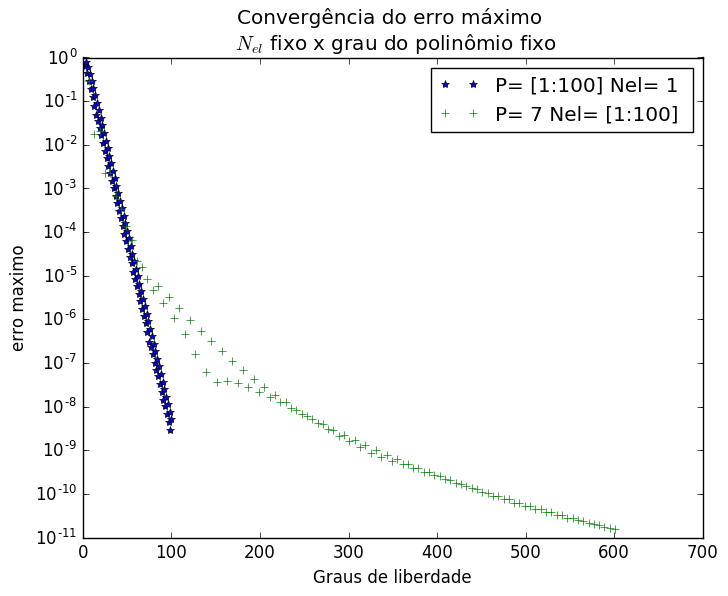
\includegraphics[width=0.5\textwidth,center]{figuras/convergencia_erro_FEM2.png}
  \caption{Convergência dos erros entre polinômios fixos e polinômios de grau elevado}
\end{figure}

\section{Método HP na resolução de equações diferenciais}

 Agora, resolveremos uma equação diferencial de segundo grau. Para tanto, irei apresentar uma equação com solução conhecida ($sin(2\ k \pi x)$. Nesse caso, definirei o problema com a condição de fronteira de \emph{Dirichlet}, definindo assim o valor nas extremidades do domínio.
\begin{align}
y'' + y &= (1 + 4 (k \pi)^2)sin(2 k \pi x) \\
y(-1) &= sin(-2\ k \ \pi ) = 0 ,\ y(1) = sin(2\ k\ \pi) = 0 \ \forall k = 1,2,\dots \\
\end{align}

\begin{figure}[!ht]
  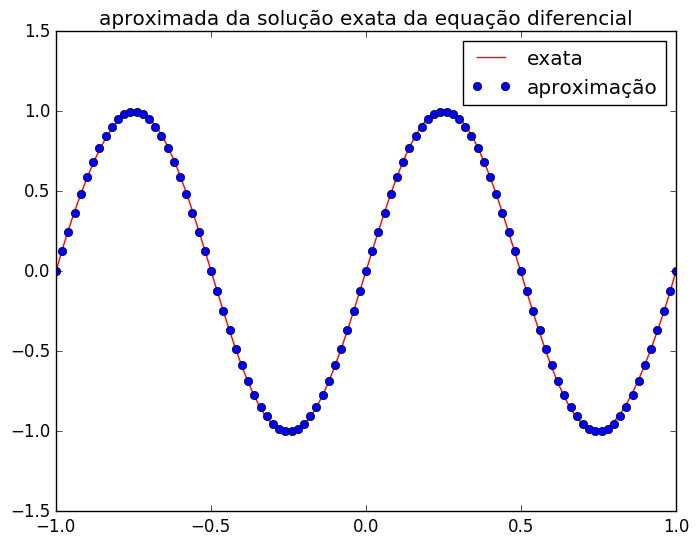
\includegraphics[width=1\textwidth,center]{figuras/solu_edo_simul.png}
  \caption{comparação entre a solução exata e a aproximada usando M= 10 e Q=10}
\end{figure}

\begin{figure}[!hb]
  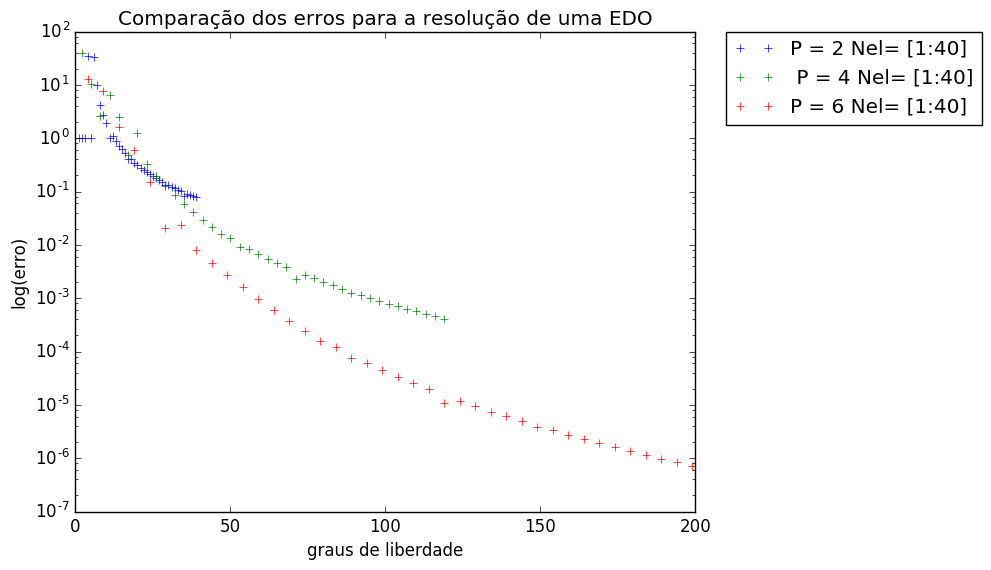
\includegraphics[width=1\textwidth,center]{figuras/convergencia_erro_EDO.png}
  \caption{convergência do log(erro) em função dos graus de liberdade fixando o grau do polinômio em P e variando o número de elementos entre 1 a 40 }
\end{figure}

\begin{table}[]
\centering
\caption{My caption}
\label{my-label}
\begin{tabular}{|l|l|}
\hline
\multicolumn{2}{|c|}{P = 2} \\ \hline
erro          & graus       \\ \hline
0.998         & 0.0         \\ \hline
1.0           & 1.0         \\ \hline
0.998         & 2.0         \\ \hline
1.0           & 3.0         \\ \hline
34.211        & 4.0         \\ \hline
1.0           & 5.0         \\ \hline
32.9996       & 6.0         \\ \hline
9.7971        & 7.0         \\ \hline
4.1311        & 8.0         \\ \hline
2.7544        & 9.0         \\ \hline
1.9603        & 10.0        \\ \hline
1.0           & 11.0        \\ \hline
1.1184        & 12.0        \\ \hline
0.8798        & 13.0        \\ \hline
0.7059        & 14.0        \\ \hline
\vdots	      & \vdots      \\
\end{tabular}
\begin{tabular}{|l|l|}
\hline
\multicolumn{2}{|l|}{P = 4} \\ \hline
erro          & graus       \\ \hline
38.8223       & 2.0         \\ \hline
10.4536       & 5.0         \\ \hline
2.6411        & 8.0         \\ \hline
6.5538        & 11.0        \\ \hline
2.4768        & 14.0        \\ \hline
0.4863        & 17.0        \\ \hline
1.2609        & 20.0        \\ \hline
0.3212        & 23.0        \\ \hline
0.1965        & 26.0        \\ \hline
0.1272        & 29.0        \\ \hline
0.085         & 32.0        \\ \hline
0.0584        & 35.0        \\ \hline
0.0409        & 38.0        \\ \hline
0.0293        & 41.0        \\ \hline
0.0214        & 44.0        \\ \hline
\vdots	      & \vdots      \\

\end{tabular}
\begin{tabular}{|l|l|}
\hline
\multicolumn{2}{|l|}{P=6} \\ \hline
erro         & graus      \\ \hline
12.9393      & 4.0        \\ \hline
7.8142       & 9.0        \\ \hline
1.6405       & 14.0       \\ \hline
0.6042       & 19.0       \\ \hline
0.1529       & 24.0       \\ \hline
0.0209       & 29.0       \\ \hline
0.0232       & 34.0       \\ \hline
0.0082       & 39.0       \\ \hline
0.0046       & 44.0       \\ \hline
0.0027       & 49.0       \\ \hline
0.0016       & 54.0       \\ \hline
0.001        & 59.0       \\ \hline
0.0006       & 64.0       \\ \hline
0.0004       & 69.0       \\ \hline
0.0002       & 74.0       \\ \hline
\vdots	      & \vdots      \\
\end{tabular}
\end{table}
